\documentclass[journal]{IEEEtran}
\usepackage{amsmath}
\usepackage{gensymb}
\usepackage{graphicx} % Required for inserting images
\usepackage{tabularx}
\usepackage{listings} 
\usepackage{ltablex}
\usepackage{upgreek}
\usepackage{multirow}
\usepackage{hyperref}
\usepackage{float}

\begin{document}

\begin{center}
   \Large Garden Automated Rain/Daylight Executed by Near-Infrared Sensing \break

   \large Nicholas Chitty, Brendan College, Scott Peirce, Justin Pham-Trinh \break

   \large University of Central Florida, Dept. of Electrical and Computer Engineering, Orlando,
   Florida, 32816-2450
\end{center}

\begin{abstract}
   Advances in both electronics and optoelectronics have greatly increased the accessibility
of complex devices. This paper will demonstrate the feasibility of installing a near infrared
scanning spectrometer into any yard, garden, or greenhouse for soil characterization with no need
for infrastructure to support it, except a water hose. Self-sufficiency will be achieved through solar
energy collection and battery storage. System control will be achieved via an electronic microcontroller.
The soil characteristics measured will be Moisture Content, Phosphorous, and Carbon. This data will be
interpreted by the microcontroller to adjust the garden bed which the device is installed on and make
the data accessible to the user. 
\end{abstract}

\section{Introduction}
\IEEEPARstart{S}{o}il characterization is shifting away from laboratory analysis and toward optical
sensing. While chemistry experiments may determine soil composition with high degrees of accuracy,
they are unfeasible on economies of scale. Every sample must be preserved for a trip back to the lab,
and lab work takes time and other valuable resources to evaluate even a single sample. Some lab work
can be done in the field, but this limits the accuracy and types of elements that can be investigated.
Spectral sensing offers two advantages: results returned by devices are limited only by scanning speeds
and computing power, and scanning covers a lot of ground, rather than a small spot. There is now a
market for precision agricultural technology, and research is ongoing to improve the efficiency of
these devices.

Soil Scanners, like those developed by AgroCares, MertControl Group, and NPC Agro, typically employ
a broadband light source to probe the soil, then collect reflectance data using an array of photodetectors.
Relevant spectral data is mostly contained within the near and mid infrared regimes. However, Moisture
Content, Carbon, Phosphorous, and pH all have spectral fingerprints that can be detected within the visible
and near infrared spectrum. A reflectance scanning spectrometer with a broadband source and one or two
cheap detectors covering the 400-1700nm range are sufficient to measure these variables.

In addition to professional products and services, hobby project forums are also advancing the
accessibility of complex systems. Hydroponic gardeners are experimenting with water distribution systems,
Arduino programmers have created a market for cheap network communication devices, and optoelectronics
hobbyists have even developed DIY optical spectrometers\cite{Cao}. These projects represent a major development in
engineering activity. It is now possible for a small, poorly funded team of amateurs to create a device
with not only mechanical function, but also wireless control and user interfacing. 

\section{Materials and Methods}

This project will integrate system controls, power, and the web, all to provide 
a "set it and forget it" home gardening experience. There are many different communication protocols
such as Bluetooth, Zigbee, Thread, and even short-range/long-range protocol. For this project we
decided to go with WiFi because of its decreased bandwidth and because we aren't expecting to produce or
receive large amounts of data. 

Another important aspect is data storage and web usage. This is important so 
that we can look back on previous information and make observations and conclusions. With our 
microcontroller, the web system is going to communicate with it through transmission control protocol.
Transmission control protocol is a standard to establish and maintain a network connection to 
exchange data. The web system will also have a 16GB database to store data and have the ability to support 
multiple garden beds in a scaled solution. As mentioned before, the web system will have a feature to 
allow the user to adjust settings but also read the data that is stored. An important factor to any 
environment is the weather and knowing when it might be cold, hot, or even rain outside. Our web system 
will communicate using HTTP requests with a weather service to receive updates that will be passed along 
to the user, when needed.

Solar power has been a growing source of energy in recent years and still continues to be with new 
developments and breakthroughs with solar technology. A lot of systems nowadays are solar powered, but 
these products are not constantly in use, they have to turn off eventually. When the product is off the 
solar panel can still collect energy which is stored in a battery for conservation. Our project will be 
the same, battery powered but charged through solar panels.

There are several means of achieving near infrared spectrometry. Our group elected to build a reflectance 
scanning spectrometer. While transmission gratings are substantially cheaper, they lose much optical power 
outside of the zero order, which is unusable due to spectral overlap. A reflectance grating will allow for 
maximum signal to noise ratio. The next challenge is how to scan. A rotational scanner was considered and 
rejected, on account of the difficulties of mechanical design. A rotating mount would have to have high 
precision movement, be rigid to ensure maintained optical alignment, and would greatly increase the 
complexity of optical alignment. A linear actuator rail with a stepper motor offered a better solution. 
Rather than change the path of the beam, it changes the position of the photodetectors along the axis of 
diffraction. This allowed for rectangular geometries, reducing the mechanical complexity of the optical 
mounts.\\

The following are the goals the team set for themselves with this project. Starting with the Primary Goals:
\begin{enumerate}
   \item A spectrometer that operates in the 400nm to 1700nm band with a spectral resolution less
         than 50nm and signal-to-noise ratio greater than 2.
   \item The ability to automatically feed water into the garden bed.
   \item Serve data to the user.
\end{enumerate}
Moving on, the team had Optional Goals:
\begin{enumerate}
   \item Power the garden bed completely from solar and battery power.
   \item Serve data to the user via a website.
\end{enumerate}
\section{High-Level Design}
Based on the goals listed above this section will discuss the high-level thought
process the team undertook in achieving those goals.
\begin{figure}[H]
    \centering
    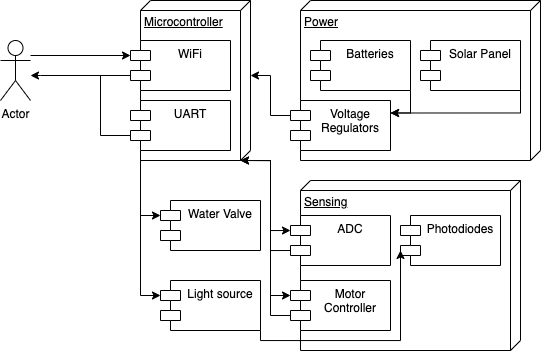
\includegraphics[width=\linewidth]{images/Flowchart.png}
    \label{fig:flowchart}
    \caption{The large systems and their interfaces and submodules}
\end{figure}
The actor is any user. The team labelled both UART and WiFi blocks as interfaces to the user
because as of the time of writing, the web server is not serving live data. In the figure, sensing is used 
interchangeably with spectrometer.
\subsection{Controller Subsystem}

% Why the MCU connects to the internet
In order for our system to be as self and power efficient as possible from an end-user perspective, our 
team decided to use a low-power, Internet-of-Things (IoT)-focused wireless microcontroller. To make the 
process of operating our product as hands-off as possible to end-users, the microcontroller will operate 
in Access Point (AP) mode to serve information to the user's mobile device. Our product will not produce 
or receive large amounts of data, or need complicated control schema for our various subsystems---and with 
power budget being a major concern of ours, our team needed to choose a product that would fit the bill.
\subsection{Spectrometer} 
The spectrometer employs a small tungsten bulb to cover the spectral range of interest. Light from the bulb 
is directed onto the soil and scattered into a fiber collimator. The collimating head couples the light into 
a fiber patch cable, which guides the light into the dark spectrometer housing. There it is reflected off a 
diffraction grating and focused onto two photodiodes. One Si photodiode covers the visible range, one InGaAs 
covers the near infrared range. These are held in position by a linear rail actuator. The current from the 
diodes is amplified and converted to voltage so that it can be detected, then the microcontroller records the 
amplitude of the signal and the position of the photodiode. The spectral data is then applied to the board logic 
for control, as well as sent to the user for display. See below for a diagram showing the path of information 
through the system.
\begin{figure}[H]
    \centering
    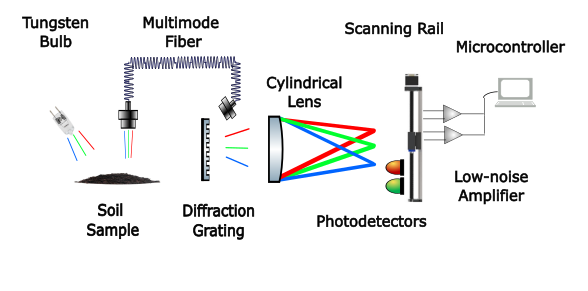
\includegraphics[width=\linewidth]{images/Schematic Diagram 2.png}
    \label{fig:sensing-block}
    \caption{Diagram showing the major components of the sensing subsystem.}
\end{figure}
\section{Major Components} \label{sec:major-components}
The components found in this section make up the logical boundaries between systems and their
subsystems.
% How the MCU connects to the internet (local network, LAN -> NAT -> WAN, TCP stack)
\subsection{Microcontroller}
The Texas Instruments CC3220-series (hence referred to as the "CC3220", the "MCU", or the "microcontroller") of microcontrollers are WiFi-enabled chips with an ARM Cortex-M4 central processor and a WiFi network processor, along with many useful peripherals and power management modules. This series of processors is delivered alongside a software development kit (SDK) provided by Texas Instruments to ease the development of IoT applications. The CC3220 is capable of running on bare metal, or with a Real-time Operating System (RTOS), allowing us to organize and schedule our various tasks.

The CC3220's WiFi network processor (NWP) supports 802.11b/g/n, SmartConfig provisioning, IPv4 and IPv6. The NWP also as the ability to host an internal HTTP/HTTPS server, and contains its own filesystem.
\subsection{Photodetectors}
When selecting a photodetector, the relevant concerns were sensitivity, effective area, and cost. Si photodiodes are cheap and reliable. Our team selected the BPX 61 by Newark, since it was the cheapest model and met our needs. The near infrared device required more careful selection. Many infrared photodetectors are used for high speed communications, with minimal surface areas and optimized rise times. Due to our concerns over signal to noise ratio, we opted for a model with a large effective area, the Thorlabs 0800-3111-011.
\subsection{Light source}
Tungsten bulbs emit a broad spectrum, far into the infrared. They also come in small package sizes that emit a lot of light for reasonable power consumption. Our bulb, the Osram 54262 runs at 20 Watts of electrical power. This is supplied directly from the battery, though controlled by the microcontroller. The result is 350 lumens, mostly directed onto the soil.
\subsection{Linear Rail}
Referring to our high-level design, the team needed a linear rail with a sled that the sensors could be mounted to.
The team found such a device on Amazon.
\subsection{Water valve}
As part of the goals, the team wanted to be able to control the flow of water
into the plant bed. To accomplish this, they chose a solenoid valve whose rated pressure was well specificied for use with home water pressures.
\section{Hardware Detail}
In \autoref{sec:major-components}, a high level overview of components and features were given. This
section will discuss the implementation details of the chosen components.
\subsection{Spectrometer}
The spectrometer is comprised of 5 major components, the photosensitive device, the linear rail and motor controller, the analog-to-digital converter, and the light source. The light source is connected via a Darlington transistor as it is driven with a 12V supply @ 1.7A. The darlington transistor will keep separate this electrical supply from the digital logic to control the lamp. The light source is fed into a fiber optic cable and pointed at a patch of soil which will reflect light into a secondary fiber optic cable.
This project involves a large diffuse source, the illumined soil. The Fiber collimator will be attached to the fiber cable via their SMA connectors, then the collimator will be set in an acrylic block so that it rests 8.06mm above the soil. The block will also have a slot for the Light source to illuminate the soil at an angle, similar to the arrangement of the source and sensor in a computer mouse above a mousepad.
The signal will travel through the fiber and up into the spectrometer housing, where the other connector of the cable will be mounted in place. Another collimator will take the output beam and collimate it so that it propagates through free space into the housing. The collimator has an output beam diameter of 1.7mm. This planar wavefront will strike the diffraction grating.
We will call to the first optic cable as the source, and the second cable as the signal. From the signal cable, the light is transmitted onto a diffraction grating. This diffraction grating will split all the wavelengths of light across a rotational area of 47\textdegree. At this point, the team can do simple trigonometry to translate a linear position to a range of wavelengths being scanned. The team chose for the sensor to be at a distance of 30mm from the diffraction grating. 
\begin{figure}[H]
    \centering
    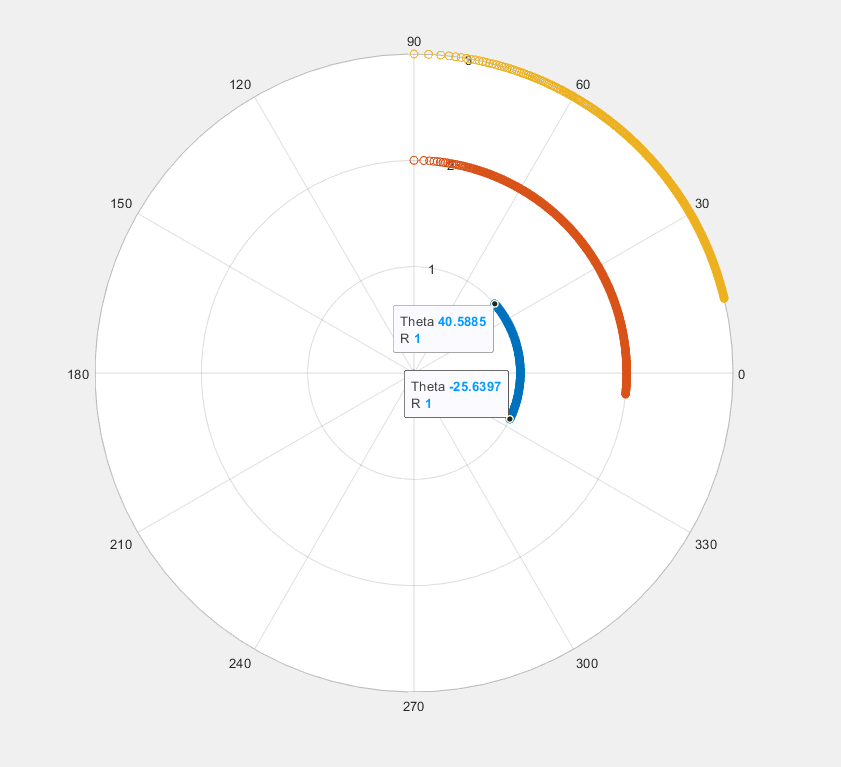
\includegraphics[width=\linewidth]{images/DiffractionAngleCalculator.png}
    \label{fig:diffraction-angle}
    \caption{The diffraction angle of 1st through 3rd order diffractions.}
\end{figure}

It is at this point that the spectrometer design enters the electrical domain. Due to the
photosensitive device being a photodiode where the current is a result of the optical power on the
sensitive area, the team built a current-to-voltage converter which would be fed into the
analog-to-digital converter. The primary issue at this point is just how small the optical power of
the light is. Given that the sensors have a translation of 1nA/1mW of power, we needed to design a
high gain, low noise converter. We chose 100e6 for the gain meaning that 1nA would translate to
100mV which is over double the resolution of our 16-bit ADC.
\begin{figure}[H]
    \centering
    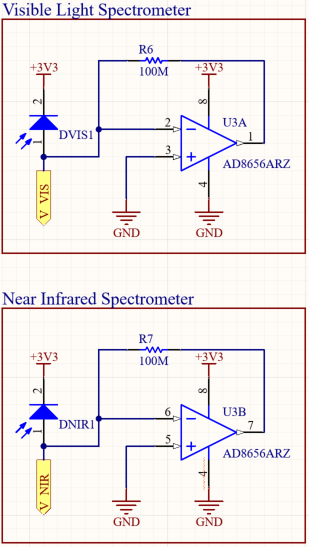
\includegraphics[height=.25\textheight]{images/SensorSchematics.PNG}
    \label{fig:sensor-schematic}
    \caption{The schematics for the current-to-voltage converter.}
\end{figure}
The net labelled \verb|V_NIR| and \verb|V_VIS| are sandwiched between ground planes on their track
to the ADC to reduce noise caused by electrostatic discharge or other analog signals (such as the
motor current). Before being read by the ADC the team designed a low pass filter to try to attenuate
the noise above 60Hz. The value of 60Hz was chosen as the cut off frequency because during
testing the oscilloscope showed a signal frequency in that range that would be detrimental to the
readings.

The sensing subsystem contains a Texas Instruments ADS 7142 ADC. The ADS 7142 is an IoT-focused nanowatt ADC with 2 external channels, an I2C interface, a sampling frequency of 140ksps, and an effective resolution of 16 bits in High-precision Mode. This ADC will be able to measure between 0 and 3.3 V from the output of the sensing subsystem's  photodiode op-amp circuit.

% How the MCU gets data from sensors (ADC, cont.)
It is expected that each photodiode's circuit will provide a voltage of between 0 and 3.3 V. The 16-bit ADC provides for an input of the same range. Therefore, the resolution of the ADC is calculated below:
\begin{equation}
    \frac{(3.3 - 0)\,\mathrm{V}}{2^{16}\,\mathrm{steps}} =
    50.35\,\mathrm{\mu V}/\mathrm{step}
\end{equation}
These steps will be used to measure OH composition and nutrients in the soil. The MCU will directly control GPIO and bit-bang values to the stepper motor controlling the position of the photodiodes allowing them to measure the full range of spectral values.
\subsection{Printed Circuit Board} Our controller subsystem was developed and implemented on a Texas Instruments LaunchPad development board. An initial control printed circuit board (PCB) was designed, fabricated, and assembled (partially seen in \ref{fig:mcu_v1_cpwg}). The chip version of the CC3220 (CC3220S) was used requiring a 4-layer impedance-controller PCB, with waveguide and external antenna, as well as oscillators, numerous bypass capacitors, and inductors. A revised PCB was designed using the module version of the CC3220 (CC3220MODAS). The PCB design was simplified, requiring only a few bypass capacitors instead of the numerous other components to support the microcontroller found on the first revision of the board.

\begin{figure}[H]
    \centering
    \label{fig:mcu_v1_cpwg}
    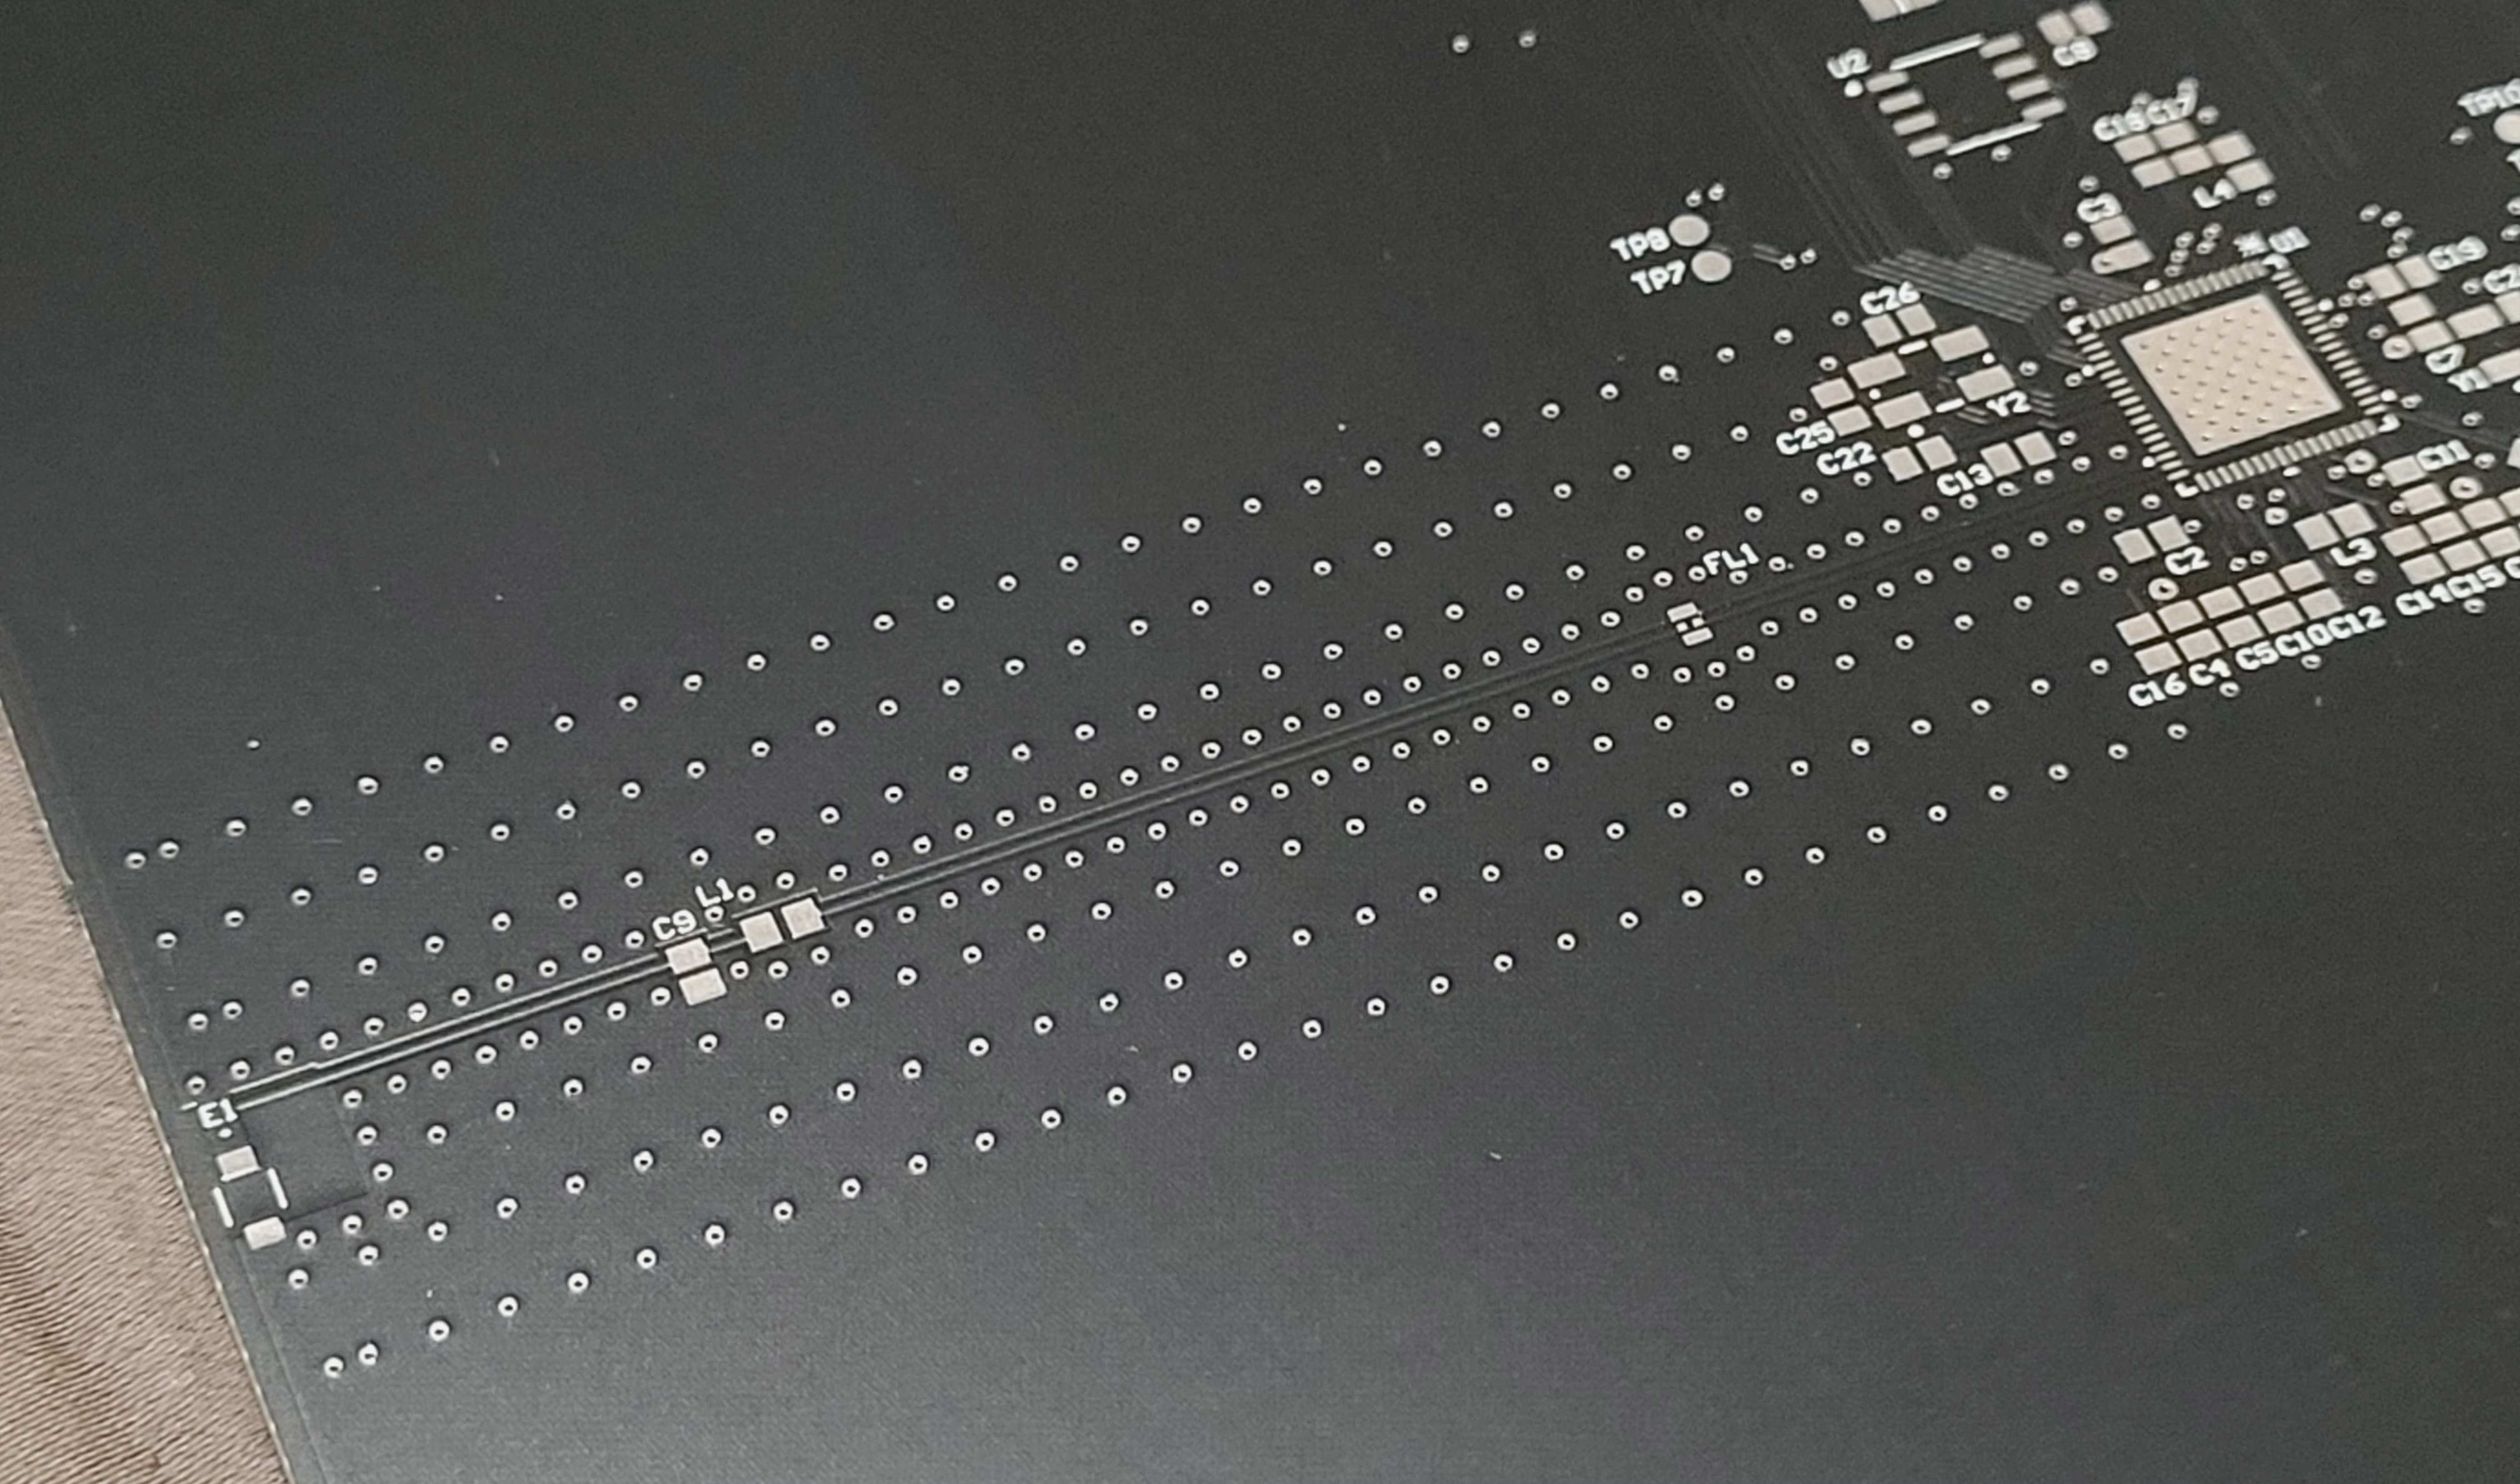
\includegraphics[width=\linewidth]{images/mcu_v1_cpwg.jpg}
    \caption{The coplanar waveguide designed to carry a 2.4 GHz signal surrounded by via fencing.}
\end{figure}
\section{Software Detail}
The microntroller serves as the glue holding this design together. In this section the means of
integrating the various subsystems via software will be discussed.
\subsection{Development Model}
An Agile development model was used to program the control subsystem and its various modules. Code reviews were performed on an as-needed basis by a convening of members of the MCU subsystem and the web subsystem teams. Texas Instruments Code Composer Studio v12 was used to program, compile (via TI ARM compiler v20), and debug the C++-based project. GitHub was used as a repository for the project, using GNU Git for version control.

The Meyers' Singleton design pattern was used for most of the classes found in our project repository (e.g. for our water solenoid class as seen in \ref{fig:singleton_implementation}). Because our team is using a RTOS with a scheduler and threads, we are using that to our advantage to divide and schedule tasks for the different submodules of our project. However, one problem our team took into consideration is that there is was only one physical instance of each submodule. The normal Singleton pattern traditionally has been used when one wants only one instance of a class initialized at any one point, but they are not thread-safe. One variation of this pattern is the Meyers' Singleton, which guarantees that only one instance of a type is available at any time. Initialization of this pattern is thread-safe, and locks can be used to ensure thread safety when accessing members of the class. This is accomplished by using a static local variable inside a static member function to hold a single instance of the class. The Meyers' Singleton takes advantage of the fact that the initialization of static local variables inside functions is guaranteed to be thread-safe. The Meyers' Singleton disallows copying and moving of the class, and makes member constructors and destructors private.

% Code style
\lstdefinestyle{mystyle}{
    basicstyle=\ttfamily\footnotesize,
    breakatwhitespace=false,         
    breaklines=true,                 
    captionpos=b,                    
    keepspaces=true,                 
    numbers=left,                    
    numbersep=-15pt,                  
    showspaces=false,                
    showstringspaces=false,
    showtabs=false,                  
    tabsize=2
}
\lstset{style=mystyle}

\begin{figure}
    \centering
    \label{fig:singleton_implementation}

\begin{lstlisting}[language=C++]
    class Water { 
        public:
            static Water& instance();

            // Disallow copying
            Water& operator = (const Water&) = delete;
            Water(const Water&) = delete;

            // Disallow moving
            Water& operator = (Water&&) = delete;
            Water(Water&&) = delete;

            // Class functions
        
        private:
            Water();
            ~Water();

            // Class variables
    };
\end{lstlisting}
\caption{An example of the Meyers' Singleton pattern implementation within the project.}
\end{figure}
\subsection{Data} As well as being able to see and configure the network settings of the product, the user will be able to see data relating to the OH-levels and common plant nutrient levels as determined by the spectral analysis of the product. For one measurement, our team will need to store 16 bits of data per position from 130 unique positions, per sensor.
\begin{equation}
    \frac{16\,\mathrm{b}}{8\,\mathrm{b/B}}\times 130\,\mathrm{positions} \times 2\,\mathrm{sensors} = 520\,\mathrm{B}
\end{equation}
With 8 Mb of the 32 Mb (1 MiB of the 4 MiB) shared serial flash dedicated to storing results, this allows us to store 2016 measurements.
\begin{equation}
    \frac{1\,\mathrm{MiB}}{520\,\mathrm{B/measurement}} = 2016\,\mathrm{measurements}
\end{equation}
Stretching out measurements to be recorded every 15 minutes, this will allow a user to see individual measurements stretching back exactly three weeks.
\begin{equation}
    2016\,\mathrm{measurements} \times \frac{1\,\mathrm{measurement}}{15\,\mathrm{min}} = 30240\,\mathrm{min} 
\end{equation}
As a stretch goal these measurements can be aggregated and analyzed, and allow us to serve trends and predictions to the user.

\subsection{Low Power Modes} The system shall run in active mode between sunrise and sunset, while the battery has 40-100\% calculated charge remaining. The system shall run in low power mode between sunrise and sunset while the battery has 10-40\% calculated charge remaining, and between sunset and sunrise while the battery has 10-100\% calculated charge remaining. The system shall run in critical power mode while the battery has 5-10\% calculated charge remaining. The system shall be in shutdown mode while the battery has 0-5\% calculated charge remaining. The system shall be able to switch power modes within 5 seconds of the interrupt being triggered.

\subsection{Connection}
Our product shall be able to broadcast a WLAN in AP mode. This will allow the user to connect to the product's SSID. The user would then be directed to a web portal hosted by the MCU's internal HTTP server, where they will be able to view information and telemetry related to the product. Hosting a web interface would allow unanimous adaptation of our product for home users. The system shall be able to broadcast a WLAN in AP mode with a nominal signal strength of 6 dBm measured at the antenna. The network shall adhere to the standards of 802.11b, g, or n. 

\subsection{Libraries}
It should be expected that the C++ standard library (as defined in C++14) will be used, as well as the POSIX library, along with the Texas Instruments SimpleLink CC32xx SDK.

% Parameters for connection and how often it tries
\subsection{Weather API Implementation}
As a stretch goal, the user will be able to configure the MCU in Station mode to allow it to connect to the user's home WLAN's SSID as a client. The user would still be able to access the MCU's web portal and see the same information as they had before. In addition, the MCU would be able to access an API to receive weather information and inform the user of recommended actions pertaining to their garden bed (e.g. if the system determines there will be freezing temperatures overnight, it may suggest to the user to cover the garden bed with a sheet or towel).
\subsection{Motor Controller}
Four GPIO lines will be used to control the stepper motor holding the sensing PCB (which includes the photodiodes, op-amp circuitry, ADC, motor controller, and connector). Depending on the digital values passed to the motor controller, the motor controller is able to control the movement direction and speed. Our team found that using the SimpleLink SDK's high-level hardware abstraction layer (HAL) provides too long of a delay when changing values in the four GPIO lines. Nanosecond-levels of delay were needed, rather than the microsecond levels of delay our team was seeing. Instead of using highly-abstracted APIs for control of the motor, our team got as close to hardware as is possible with C/C++ and used TI's driverlib driver library specifically for the CC3220. Instead of a simple GPIO number being passed to the function, our team had to determine the GPIO port and port-specific pin of each input of our motor controller. The driverlib function checks the port for correctness, and then performs a system call to write a value directly to memory (in our case, the address of the GPIO port). Using driverlib also allows us to bit stuff our GPIO pins if they are located on the same port---in our second iteration of the board, the motor controller GPIOs were relocated to the same GPIO port and bitmasks used so we can change all four GPIO pins with one driverlib write function. This allows us to toggle a single GPIO pin within a period of 350 ns (seen in \ref{fig:gpio_toggle_driverlib}). With a speed of 80 MHz in active mode, this would mean we're able to write to GPIO in only 28 processor cycles.
\begin{equation}
    350\,\mathrm{ns} \times (80\times10^6\mathrm{cycles/s}) = 28\,\mathrm{cycles}
\end{equation}
This is a huge accomplishment for our team, especially with a program written in C++ and utilizing HAL.

\begin{figure}[H]
    \centering
    \label{fig:gpio_toggle_driverlib}
    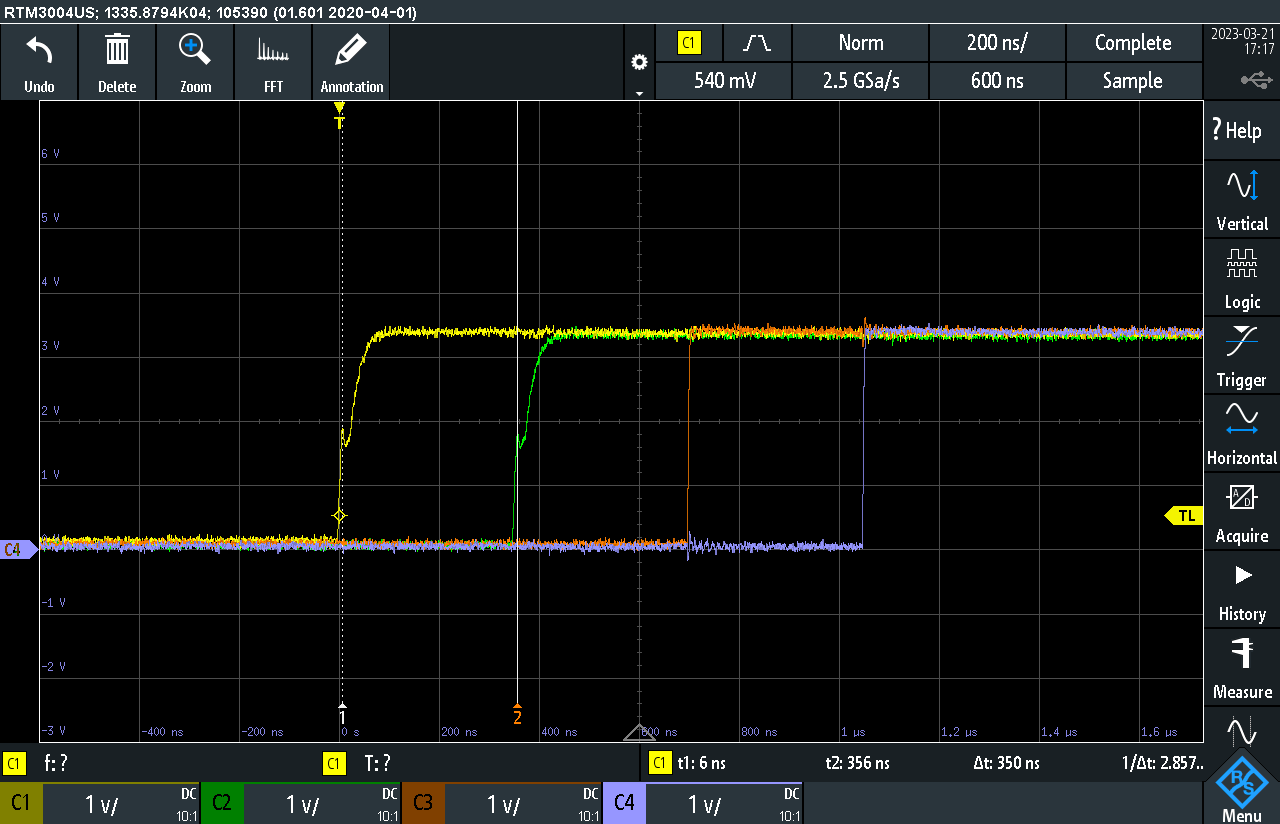
\includegraphics[width=\linewidth]{images/gpio_toggle_driverlib.jpg}
    \caption{Toggling GPIO using driverlib results in a very short (350 ns) delay.}
\end{figure}
To drive a DC motor we similarly needed a device to separate the digital logic from the back emf of the motor. This is done through the use of the motor driver. The timing of the signals is the most important part as the driver is just using the current and voltage source designed specifically for the motor in the timings given by the input pins. Wrong timing leads to the ability to skip tests leading to indeterministic behavior. The issue is the the CC32xx SDK abstracts away a lot of the fine tunability of setting hardware registers. To resolve this, the team used the specific board's hardware driver implementation to set the output on the pins with a delay of only 28 cycles.
\subsection{Over-the-Air Updates}
At this time, our team does not intend to provide a method for over-the-air updates (OTA), however, this is a stretch goal that may be completed in the future.

\subsection{Startup and Shutdown} Startup and shutdown will occur in a timely manner (within seconds). Abrupt shutdown shall not damage any components of the system, and the system will be able to restart to its previous state without any input from the user. If the system freezes or crashes, its internal watchdog timer will automatically reboot the device.
\bibliographystyle{ieeetr}
\bibliography{references/sensing}
\end{document}